\subsection{Angular relationships} \label{sec:angular_relationships}
Before the energy yield of a PV generator can be calculated, it is essential to introduce a few important angles -- of which some were already mentioned -- and define how they are counted in this thesis.

The local latitude $\varphi$ at the equator is $0^\circ$ and it is counted positive towards the north and negative towards the south with a range of $\left[-90^\circ \text{, } 90^\circ\right]$, and the local \emph{longitude} $\lambda$ in $\left(^\circ\right)$ is $0^\circ$ at the reference meridian $\lambda_0$ in $\left(^\circ\right)$ which passes through the Greenwich Observatory in the United Kingdom. $\lambda$ is counted positive east and negative west of Greenwich with a range of $\left(-180^\circ \text{, } 180^\circ\right]$ \cite{Landis:1995, Karttunen:2006, Wagner:2018}. For completens it should be mentioned that the latitude $\varphi$ and the longitude $\lambda$ -- for a given location on Earth -- can be obtained from an atlas or a \emph{global positioning system} (GPS) device.

The Sun's declination $\delta$ indicates how far the Earth's axis of rotations -- which runs through the North and South Poles -- leans towards the Sun at solar noon. Its range is $\left[-90^\circ \text{, } 90^\circ\right]$, although its maximum values for Earth are $-23,45^\circ$ and $23,45^\circ$. $\delta$ is counted negative if the North Pole leans away from the Sun and positive if it leans towards the Sun (compare to figure \ref{fig:tikz_angular_relationship}) \cite{Landis:1995, Karttunen:2006, Mertens:2015, Wagner:2018}. As per \cite{Wagner:2018}, the following approximation for $\delta$ at a given day of the year, with $N_d$ being the \emph{number of days} since January 1\textsuperscript{st} in $\left(\mathrm d \right)$,  $mon$ being the \emph{month} in $\left( 1 \right)$ and $d$ being the \emph{day} in $\left(\mathrm d \right)$, is sufficient for photovoltaic applications: 
	\begin{equation} \label{eq:delta}
	\centering
		\delta \approx 23,45^\circ \cdot \sin \left(360^\circ \cdot \frac{284\mathrm{d} + N_d}{365\mathrm{d}}\right) \text{,} 
	\end{equation}
	\begin{equation} \label{eq:delta}
	\centering
		N_d \approx 30,3\mathrm{d} \cdot \left(mon - 1\right) + d \text{.}
	\end{equation}

The altitude $\gamma_{\mathrm{S}}$ and the \emph{azimuth} $\alpha_{\mathrm{S}}$ of the Sun in $\left(^\circ \right)$, presented in the equations (\ref{eq:sin_gamma_s}) and (\ref{eq:cos_alpha_s}), describe its position in the sky over the course of the day, with $\gamma_{\mathrm{S}}$ taking on values within $\left[0^\circ \text{, } 90^\circ\right]$ and $\alpha_{\mathrm{S}}$ taking on values within $\left(-180^\circ \text{, } 180^\circ \right]$. How these angles are measured -- with the corresponding celstial hemisphere of an observer -- is shown in the figure \ref{fig:tikz_gamma_s_alpha_s}. For $\gamma_{\mathrm{S}} = 0^\circ$ the Sun is visible at the horizon and for $\gamma_{\mathrm{S}} = 90^\circ$ it is visible at its zenith. For $\alpha_{\mathrm{S}} = 0^\circ$ the Sun is visible exactly in the south. $\alpha_{\mathrm{S}}$ takes on positive values towards the west and negative values towards the east \cite{Landis:1995, Karttunen:2006, Mertens:2015, Wagner:2018}.
	\begin{equation} \label{eq:sin_gamma_s}
	\centering
		\sin \gamma_{\mathrm{S}} = \sin \varphi \, \sin \delta + \cos \varphi \, \cos \delta \, \cos h_{\mathrm{S}}
	\end{equation}
	\begin{equation} \label{eq:cos_alpha_s}
	\centering
		\cos \alpha_{\mathrm{S}} = \frac{\sin \varphi \, \cos \delta \, \cos h_{\mathrm{S}} - \cos \varphi \, \sin \delta}{\cos \gamma_{\mathrm{S}}}
	\end{equation}
\begin{figure}[h!]
	\centering
	

\tikzset{every picture/.style={line width=0.75pt}} %set default line width to 0.75pt        

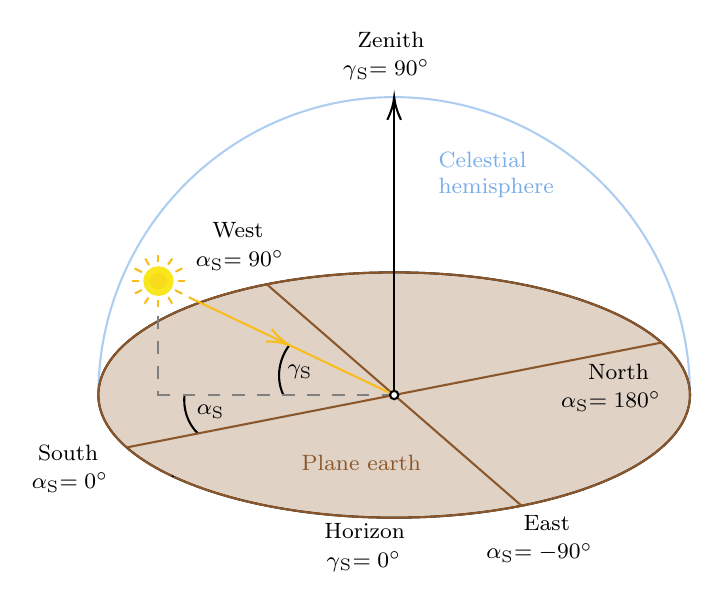
\begin{tikzpicture}[x=0.75pt,y=0.75pt,yscale=-1,xscale=1]
%uncomment if require: \path (0,445); %set diagram left start at 0, and has height of 445






%Shape: Ellipse [id:dp10248886204350427] 
\draw  [color={rgb, 255:red, 0; green, 0; blue, 0 }  ,draw opacity=1 ][fill={rgb, 255:red, 139; green, 87; blue, 42 }  ,fill opacity=0.27 ] (120.55,216.48) .. controls (120.55,183.84) and (184.36,157.39) .. (263.08,157.39) .. controls (341.79,157.39) and (405.61,183.84) .. (405.61,216.48) .. controls (405.61,249.12) and (341.79,275.58) .. (263.08,275.58) .. controls (184.36,275.58) and (120.55,249.12) .. (120.55,216.48) -- cycle ;
%Shape: Arc [id:dp9824695676563142] 
\draw  [draw opacity=0] (120.55,216.48) .. controls (120.55,216.48) and (120.55,216.48) .. (120.55,216.48) .. controls (120.55,137.22) and (184.36,72.96) .. (263.08,72.96) .. controls (341.79,72.96) and (405.61,137.22) .. (405.61,216.48) -- (263.08,216.48) -- cycle ; \draw  [color={rgb, 255:red, 74; green, 144; blue, 226 }  ,draw opacity=0.45 ] (120.55,216.48) .. controls (120.55,216.48) and (120.55,216.48) .. (120.55,216.48) .. controls (120.55,137.22) and (184.36,72.96) .. (263.08,72.96) .. controls (341.79,72.96) and (405.61,137.22) .. (405.61,216.48) ;
%Shape: Ellipse [id:dp6726138734461271] 
\draw  [color={rgb, 255:red, 248; green, 231; blue, 28 }  ,draw opacity=1 ][fill={rgb, 255:red, 248; green, 220; blue, 28 }  ,fill opacity=1 ][line width=2.25]  (143.71,161.61) .. controls (143.71,158.48) and (146.3,155.95) .. (149.5,155.95) .. controls (152.7,155.95) and (155.3,158.48) .. (155.3,161.61) .. controls (155.3,164.73) and (152.7,167.27) .. (149.5,167.27) .. controls (146.3,167.27) and (143.71,164.73) .. (143.71,161.61) -- cycle ;
%Straight Lines [id:da22837958638990763] 
\draw [color={rgb, 255:red, 248; green, 189; blue, 28 }  ,draw opacity=1 ]   (149.5,148.94) -- (149.5,152.47) ;
%Straight Lines [id:da36410436567305116] 
\draw [color={rgb, 255:red, 248; green, 189; blue, 28 }  ,draw opacity=1 ]   (162.47,161.61) -- (158.86,161.61) ;
%Straight Lines [id:da7784535438011968] 
\draw [color={rgb, 255:red, 248; green, 189; blue, 28 }  ,draw opacity=1 ]   (149.5,174.27) -- (149.5,170.75) ;
%Straight Lines [id:da02148874103533327] 
\draw [color={rgb, 255:red, 248; green, 189; blue, 28 }  ,draw opacity=1 ]   (140.14,161.61) -- (136.53,161.61) ;
%Straight Lines [id:da5806655094182651] 
\draw [color={rgb, 255:red, 248; green, 189; blue, 28 }  ,draw opacity=1 ]   (157.5,165.91) -- (160.98,167.72) ;
%Straight Lines [id:da9042107417993022] 
\draw [color={rgb, 255:red, 248; green, 189; blue, 28 }  ,draw opacity=1 ]   (138.03,155.49) -- (141.5,157.31) ;
%Straight Lines [id:da8739850131703888] 
\draw [color={rgb, 255:red, 248; green, 189; blue, 28 }  ,draw opacity=1 ]   (160.98,155.49) -- (157.7,157.08) ;
%Straight Lines [id:da9973855947966144] 
\draw [color={rgb, 255:red, 248; green, 189; blue, 28 }  ,draw opacity=1 ]   (141.5,165.91) -- (138.23,167.49) ;
%Straight Lines [id:da23606504338204548] 
\draw [color={rgb, 255:red, 248; green, 189; blue, 28 }  ,draw opacity=1 ]   (154.14,153.67) -- (156.11,150.74) ;
%Straight Lines [id:da06728456263139648] 
\draw [color={rgb, 255:red, 248; green, 189; blue, 28 }  ,draw opacity=1 ]   (142.78,172.46) -- (144.75,169.53) ;
%Straight Lines [id:da5070173352082208] 
\draw [color={rgb, 255:red, 248; green, 189; blue, 28 }  ,draw opacity=1 ]   (154.26,169.3) -- (156.11,172.47) ;
%Straight Lines [id:da536701929565258] 
\draw [color={rgb, 255:red, 248; green, 189; blue, 28 }  ,draw opacity=1 ]   (143.13,150.74) -- (144.98,153.91) ;
%Straight Lines [id:da1832197332832679] 
\draw [color={rgb, 255:red, 139; green, 87; blue, 42 }  ,draw opacity=1 ]   (324.28,269.67) -- (263.08,216.48) ;
%Straight Lines [id:da35722852927602045] 
\draw [color={rgb, 255:red, 139; green, 87; blue, 42 }  ,draw opacity=1 ]   (263.08,216.48) -- (201.88,163.3) ;
%Shape: Arc [id:dp6576066040432391] 
\draw  [draw opacity=0] (168.58,235.07) .. controls (163.53,230.23) and (161.29,223.2) .. (162.06,216.13) -- (185.16,216.91) -- cycle ; \draw   (168.58,235.07) .. controls (163.53,230.23) and (161.29,223.2) .. (162.06,216.13) ;
%Shape: Arc [id:dp8644885498360859] 
\draw  [draw opacity=0] (209.82,216.7) .. controls (206.04,209.04) and (207.21,199.65) .. (212.57,192.43) -- (231.46,205.17) -- cycle ; \draw   (209.82,216.7) .. controls (206.04,209.04) and (207.21,199.65) .. (212.57,192.43) ;
%Straight Lines [id:da40176543382530383] 
\draw [color={rgb, 255:red, 248; green, 189; blue, 28 }  ,draw opacity=1 ]   (263.08,216.48) -- (212.58,192.42) ;
%Straight Lines [id:da43066607290523007] 
\draw [color={rgb, 255:red, 128; green, 128; blue, 128 }  ,draw opacity=1 ] [dash pattern={on 4.5pt off 4.5pt}]  (149.15,216.48) -- (263.08,216.48) ;
%Straight Lines [id:da9460200323685761] 
\draw [color={rgb, 255:red, 139; green, 87; blue, 42 }  ,draw opacity=1 ]   (133.86,241.81) -- (263.08,216.48) ;
%Straight Lines [id:da12611331746579268] 
\draw [color={rgb, 255:red, 139; green, 87; blue, 42 }  ,draw opacity=1 ]   (263.08,216.48) -- (392.3,191.15) ;
%Shape: Arc [id:dp7682340536128898] 
\draw  [draw opacity=0] (155.96,255.47) .. controls (133.92,245.06) and (120.55,231.42) .. (120.55,216.48) .. controls (120.55,183.84) and (184.36,157.39) .. (263.08,157.39) .. controls (341.79,157.39) and (405.61,183.84) .. (405.61,216.48) .. controls (405.61,249.12) and (341.79,275.58) .. (263.08,275.58) .. controls (220.87,275.58) and (182.95,267.97) .. (156.85,255.88) -- (263.08,216.48) -- cycle ; \draw  [color={rgb, 255:red, 139; green, 87; blue, 42 }  ,draw opacity=1 ] (155.96,255.47) .. controls (133.92,245.06) and (120.55,231.42) .. (120.55,216.48) .. controls (120.55,183.84) and (184.36,157.39) .. (263.08,157.39) .. controls (341.79,157.39) and (405.61,183.84) .. (405.61,216.48) .. controls (405.61,249.12) and (341.79,275.58) .. (263.08,275.58) .. controls (220.87,275.58) and (182.95,267.97) .. (156.85,255.88) ;
%Straight Lines [id:da15722411504245715] 
\draw [color={rgb, 255:red, 128; green, 128; blue, 128 }  ,draw opacity=1 ] [dash pattern={on 4.5pt off 4.5pt}]  (149.5,178.56) -- (149.5,216.93) ;
%Straight Lines [id:da003502427569964439] 
\draw [color={rgb, 255:red, 248; green, 189; blue, 28 }  ,draw opacity=1 ]   (210.77,191.57) -- (164.08,169.36) ;
\draw [shift={(212.57,192.43)}, rotate = 205.44] [color={rgb, 255:red, 248; green, 189; blue, 28 }  ,draw opacity=1 ][line width=0.75]    (10.93,-3.29) .. controls (6.95,-1.4) and (3.31,-0.3) .. (0,0) .. controls (3.31,0.3) and (6.95,1.4) .. (10.93,3.29)   ;
%Straight Lines [id:da8840339574734517] 
\draw    (263.08,216.48) -- (263.08,74.96) ;
\draw [shift={(263.08,72.96)}, rotate = 450] [color={rgb, 255:red, 0; green, 0; blue, 0 }  ][line width=0.75]    (10.93,-3.29) .. controls (6.95,-1.4) and (3.31,-0.3) .. (0,0) .. controls (3.31,0.3) and (6.95,1.4) .. (10.93,3.29)   ;
%Shape: Circle [id:dp5710959149747352] 
\draw  [fill={rgb, 255:red, 255; green, 255; blue, 255 }  ,fill opacity=1 ] (261.08,216.48) .. controls (261.08,215.38) and (261.97,214.48) .. (263.08,214.48) .. controls (264.18,214.48) and (265.08,215.38) .. (265.08,216.48) .. controls (265.08,217.59) and (264.18,218.48) .. (263.08,218.48) .. controls (261.97,218.48) and (261.08,217.59) .. (261.08,216.48) -- cycle ;

% Text Node
\draw (210.29,200.68) node [anchor=north west][inner sep=0.75pt]  [font=\footnotesize]  {$\gamma _{\mathrm{S}}$};
% Text Node
\draw (166.49,219.8) node [anchor=north west][inner sep=0.75pt]  [font=\footnotesize]  {$\alpha _{\mathrm{S}}$};
% Text Node
\draw (217,244) node [anchor=north west][inner sep=0.75pt]  [font=\footnotesize,color={rgb, 255:red, 139; green, 87; blue, 42 }  ,opacity=1 ] [align=left] {Plane earth};
% Text Node
\draw (87,252.4) node [anchor=north west][inner sep=0.75pt]  [font=\footnotesize]  {$\textcolor[rgb]{0,0,0}{\alpha }\textcolor[rgb]{0,0,0}{_{\mathrm{S}}}\textcolor[rgb]{0,0,0}{=0}\textcolor[rgb]{0,0,0}{^{\circ }}$};
% Text Node
\draw (90,239) node [anchor=north west][inner sep=0.75pt]  [font=\footnotesize] [align=left] {South};
% Text Node
\draw (324,273) node [anchor=north west][inner sep=0.75pt]  [font=\footnotesize] [align=left] {East};
% Text Node
\draw (306,286.4) node [anchor=north west][inner sep=0.75pt]  [font=\footnotesize]  {$\textcolor[rgb]{0,0,0}{\alpha }\textcolor[rgb]{0,0,0}{_{\mathrm{S}}}\textcolor[rgb]{0,0,0}{=-90}\textcolor[rgb]{0,0,0}{^{\circ }}$};
% Text Node
\draw (244,40) node [anchor=north west][inner sep=0.75pt]  [font=\footnotesize] [align=left] {Zenith};
% Text Node
\draw (237,53.4) node [anchor=north west][inner sep=0.75pt]  [font=\footnotesize]  {$\textcolor[rgb]{0,0,0}{\gamma }\textcolor[rgb]{0,0,0}{_{\mathrm{S}}}\textcolor[rgb]{0,0,0}{=90}\textcolor[rgb]{0,0,0}{^{\circ }}$};
% Text Node
\draw (174,132) node [anchor=north west][inner sep=0.75pt]  [font=\footnotesize] [align=left] {West};
% Text Node
\draw (166,145.4) node [anchor=north west][inner sep=0.75pt]  [font=\footnotesize]  {$\textcolor[rgb]{0,0,0}{\alpha }\textcolor[rgb]{0,0,0}{_{\mathrm{S}}}\textcolor[rgb]{0,0,0}{=90}\textcolor[rgb]{0,0,0}{^{\circ }}$};
% Text Node
\draw (342,213.4) node [anchor=north west][inner sep=0.75pt]  [font=\footnotesize]  {$\textcolor[rgb]{0,0,0}{\alpha }\textcolor[rgb]{0,0,0}{_{\mathrm{S}}}\textcolor[rgb]{0,0,0}{=180}\textcolor[rgb]{0,0,0}{^{\circ }}$};
% Text Node
\draw (355,200) node [anchor=north west][inner sep=0.75pt]  [font=\footnotesize] [align=left] {North};
% Text Node
\draw (229,290.4) node [anchor=north west][inner sep=0.75pt]  [font=\footnotesize]  {$\textcolor[rgb]{0,0,0}{\gamma }\textcolor[rgb]{0,0,0}{_{\mathrm{S}}}\textcolor[rgb]{0,0,0}{=0}\textcolor[rgb]{0,0,0}{^{\circ }}$};
% Text Node
\draw (228,277) node [anchor=north west][inner sep=0.75pt]  [font=\footnotesize] [align=left] {Horizon};
% Text Node
\draw (283,98) node [anchor=north west][inner sep=0.75pt]  [font=\footnotesize,color={rgb, 255:red, 74; green, 144; blue, 226 }  ,opacity=0.74 ] [align=left] {Celestial\\hemisphere};


\end{tikzpicture}

	\caption{Angular relationship of the Sun's altitude $\gamma_{\mathrm{S}}$ and azimuth $\alpha_{\mathrm{S}}$ with the corresponding celestial hemisphere of an observer. In this figure the Sun already passed the solar noon. (Recreated from: \cite{Mertens:2015})}
	\label{fig:tikz_gamma_s_alpha_s}
\end{figure}

It must be noted that $\gamma_{\mathrm{S}}$ and $\alpha_{\mathrm{S}}$ change over the course of the day. By analyzing the equations (\ref{eq:sin_gamma_s}) and (\ref{eq:cos_alpha_s}), while taking into account that $\varphi$ does not change because the self-sufficient voice communication system is stationary for the entire mission and that in this thesis $\delta$ is modeled with a constant value throughout the day -- altough it takes on different values for each day of the year -- it must be the variable $h_{\mathrm{S}}$ in $\left(^\circ\right)$ that is responsible for these changes. It is called the \emph{solar hour angle} and its value is $0^\circ$ when the Sun reaches its greatest daily altitude $\gamma_{\mathrm{S}}$, which occurs at solar noon. This happens for either $\alpha_{\mathrm{S}} = 0^\circ$, $\alpha_{\mathrm{S}} = 180^\circ$ or for $\gamma_{\mathrm{S}} = 90^\circ$, where $\alpha_{\mathrm{S}}$ is undefined. $h_{\mathrm{S}}$ is counted negative before the solar noon and positive after the solar noon with a range of $\left(-180^\circ \text{, } 180^\circ\right]$. \cite{Landis:1995, Karttunen:2006, Mertens:2015, Wagner:2018}.  

For a given \emph{solar time}\footnote{In most cases the solar time $t_\mathrm{S}$ differs from the local time on a wrist watch. For $t_\mathrm{S} = 12\mathrm{h}$ (solar noon) the Sun is either exaclty in the south, in the north or at its zenith, whereas the Sun might not be exactly in the south, in the north or at its zenith for the \emph{local time} $t_\mathrm{local} = 12\mathrm{h}$ on a wrist watch -- no matter how accurate it is set to the local time.} $t_\mathrm{S}$ in $\left(\mathrm h \right)$, the hour angle $h_\mathrm{S}$ can be determined as shown in equation (\ref{eq:solar_hour_angle}). The factor $\frac{15^\circ}{1\mathrm{h}}$ comes about because the Earth rotates $360^\circ$ within $24\mathrm{h}$. Thus the range of the solar time $t_\mathrm{S}$ can be derived to $\left[0\mathrm{h} \text{, } 24\mathrm{h}\right)$. Further, the hour angle for the \emph{solar sunrise time} $t_\mathrm{S,r}$ in $\left(\mathrm h \right)$ and the \emph{solar sunset time} $t_\mathrm{S,s}$ in $\left(\mathrm h \right)$ can be calculated with the equations (\ref{eq:h_sunrise}) and (\ref{eq:h_sunset}) \cite{Landis:1995, Karttunen:2006, Mertens:2015, Wagner:2018}.
	\begin{equation} \label{eq:solar_hour_angle}
	\centering
		h_\mathrm{S} = \left(t_\mathrm{S} - 12\mathrm{h} \right) \cdot \frac{15^\circ}{1\mathrm{h}}
	\end{equation}
	\begin{equation} \label{eq:h_sunrise}
	\centering
		h_\mathrm{S,r} = - \arccos \left( -\tan \delta \tan \, \varphi \right) \text{,} \quad \text{for } \left|\varphi\right| < 90^\circ - \left|\delta\right|
	\end{equation}
	\begin{equation} \label{eq:h_sunset}
	\centering
		h_\mathrm{S,s} = \arccos \left( -\tan \delta \, \tan \varphi \right) \text{,} \quad \text{for } \left|\varphi\right| < 90^\circ - \left|\delta\right|
	\end{equation}

In the article \cite{Landis:1995} a few importnat cases, regarding the equations (\ref{eq:h_sunrise}) and (\ref{eq:h_sunset}), are mentioned which might be of interest when selecting a locations to install the self-sufficient voice communication system:
%\vspace{2mm}
\[ \tan \delta \, \tan \varphi \,
  \begin{cases}
    > 1       	& \text{polar night, if } \varphi < -90^\circ + \delta \text{ or } \varphi > 90^\circ + \delta \text{,} \\
    = \pm 1  		& \text{the Sun is only visible at the horizon for an instant,} \\
    < -1		& \text{polar day, if } \varphi < -90^\circ - \delta \text{ or } \varphi > 90^\circ - \delta \text{.}
  \end{cases}
\]
%\vspace{2mm}

The solar time $t_\mathrm{S}$ can finally be calculated from $t_\mathrm{UTC}$ in $\left(\mathrm h \right)$, which is the \emph{Coordinated Universal Time} (UTC), using the equation (\ref{eq:solar_time}) where $\lambda_0 = 0^\circ$ is the reference meridian for which $t_\mathrm{UTC}$ applies and $Z_{\mathrm{h}}$ in $\left(\mathrm{h}\right)$ is the \emph{equation of time} which serves as a correction factor  \cite{Karttunen:2006, Wagner:2018}.
	\begin{equation} \label{eq:solar_time}
	\centering
		t_\mathrm{S} = t_\mathrm{UTC} + Z_{\mathrm{h}} + \left(\lambda - \lambda_{\mathrm{0}}\right) \cdot \frac{1\mathrm{h}}{15\degree}
	\end{equation}
	\begin{equation} \label{eq:time_equation}
	\centering
		Z_{\mathrm{h}} \approx 0,123\mathrm{h} \cdot \cos \left(360^\circ \cdot \frac{88\mathrm{d} + N_d}{365\mathrm{d}}\right) - 0,167\mathrm{h} \cdot \sin \left(720^\circ \cdot \frac{10\mathrm{d} + N_d}{365\mathrm{d}}\right) 
	\end{equation}
